\documentclass[11pt]{article}
\usepackage[letterpaper,margin=1in]{geometry}
\usepackage[T1]{fontenc}
\usepackage{lmodern,microtype,amsmath,booktabs,tabularx,xltabular}
\usepackage{xcolor,enumitem,float,fvextra,setspace}
\usepackage[font=normalsize,labelfont=bf]{caption}
\usepackage[numbers,sort&compress]{natbib}
\usepackage{tikz,pgfplots}
\usetikzlibrary{arrows.meta,positioning,calc}
\usepgfplotslibrary{groupplots}
\pgfplotsset{compat=1.18}
\usepackage[colorlinks=true,linkcolor=blue!35!black,citecolor=blue!35!black,urlcolor=blue!50!black,breaklinks=true]{hyperref}
\hypersetup{pdftitle={Counting Reports or Counting Evidence},pdfauthor={DSA4213 Group 14},pdfsubject={Final project report}}
\newcolumntype{L}{>{\raggedright\arraybackslash}X}
\newcolumntype{P}[1]{>{\raggedright\arraybackslash}p{#1}}
\definecolor{opus}{HTML}{2167B1}
\definecolor{sonnet}{HTML}{CE5D21}
\definecolor{gpt}{HTML}{16816A}
\definecolor{muted}{HTML}{777777}
\definecolor{gridc}{HTML}{DDDDDD}
\definecolor{axisc}{HTML}{777777}
\pgfplotsset{report/.style={axis lines*=left,axis line style={axisc},tick style={axisc},ymajorgrids,grid style={gridc,line width=.4pt},tick label style={font=\normalsize},label style={font=\normalsize},title style={font=\normalsize\bfseries}}}
\setlist{itemsep=2pt,topsep=4pt}
\setlength{\emergencystretch}{2em}
\setstretch{1.10}
\setlength{\parskip}{3pt plus 1pt}
\widowpenalty=10000
\clubpenalty=10000
\raggedbottom
\newcommand{\neff}{n_{\mathrm{eff}}}
\newcommand{\pt}{\ensuremath{P(\mathrm{truth})}}
\newcommand{\pa}{P(\mathrm{A's\ claim})}
\newcommand{\repo}{https://github.com/JasonOng0109/dsa4213-agent-project}
\begin{document}
\begin{center}
{\LARGE\bfseries Counting Reports or Counting Evidence:}\\[.3em]
{\large What Provenance an LLM Orchestrator Needs\\
to Discount Correlated Agent Reports}\\[.7em]
Final report, Group 14\\
DSA4213 Natural Language Processing for Data Science\\
Semester 1, AY2026/2027\\[.7em]
Ong Jia Xi (A0276092Y) \quad Lee Kai Rong (A0287723U)\\
Kathleen Pang Qi Yu (A0282219A) \quad Ee Rui Kai Rachel (A0281201X)\\
Crystal Lai Qiaohui (A0282431L)
\end{center}
\noindent\textbf{Project direction:} Provenance-aware aggregation of agent reports.\\
\textbf{Repository:} \href{\repo}{Code, data and project materials}.
\section*{Project summary}
\noindent Multi-agent systems often give one model, the orchestrator, the reports of several worker agents. Workers that share a retriever or a tool can pass on the same source. In 40 cases with invented facts, a separate reporter model rewords each source and the accepted reports are frozen. Three judges gave an answer and a probability for every option in 20,280 trials. With nothing disclosed, two reports of a weak source beat one report of a strong source in 454 to 479 of 480 trials per judge. Told that two reports share a source, every judge raised its stated probability of the truth in at least 37 of 40 cases, yet stayed wrong in most trials. Told which source is the primary record, every judge was right in every trial. Even ``somewhat more reliable'' was enough in 331 of 360 subset trials. Every note we showed was true, so this does not establish robustness to false quality labels.

\section{Introduction}
\label{sec:intro}
Many language-model systems split a task across worker agents and give one model, the orchestrator, the job of combining what the workers report. Workers in one framework often share a retriever or a tool, so their reports can be correlated by construction. Consider three workers that receive the same document and each summarise it in their own words. The reports look like three witnesses, but only one source exists.

A multi-agent system holds the information that could prevent this failure, because it knows which agent called which tool and which document came back. That record is lost when the workers' outputs are rendered as text for the orchestrator. Our research question is the following.
\begin{quote}\itshape
Can the orchestrator distinguish the number of agreeing reports from the number and quality of the independent sources behind them, and what must the inter-agent message tell it (a source ID, a source type, that reports share a source, or which source is more reliable) before its belief and its decision follow the evidence?
\end{quote}
We make four contributions. We compare disclosures on identical frozen reports, measure belief and choice side by side with an abstention arm, build a corpus of independently generated paraphrases with provenance kept out of the text, and adapt an index that estimates how many independent sources a judge behaves as if it saw. ``Belief'' here means stated probability, not calibrated or internal belief. Success means interpretable evidence about the primary hypotheses, including negative results.

After the TA's feedback, we reworded the question to name the aggregation step and the lost source record. The design was unchanged. Post-pilot changes to the screen and abstention controls are documented in Appendix~\ref{app:departures}.

\section{Related work}
\label{sec:related}
\citet{xu2024survey} separate conflicts between supplied evidence from conflicts with a model's own knowledge. Our setting is the first kind, while ClashEval studies the second~\citep{wu2024clasheval}. We remove that axis by using invented entities throughout. \citet{schuster2026whose} find a credibility hierarchy that repetition can reverse. Their repeated evidence is verbatim. RAMDocs gives each document its own agent, so count and independence cannot be separated~\citep{wang2025ramdocs}. AuthorityBench studies authority from URLs~\citep{yao2026authoritybench}.

Multi-agent debate treats agreeing outputs as corroboration~\citep{du2023debate}. Minority Sentinel trains a classifier to overturn wrong majorities~\citep{he2026minority}, while conformity and sycophancy can push debate toward consensus~\citep{cui2025freemad,yao2025sycophancy}. Our agents never interact, and their agreement is inherited from the source. Provenance-aware memory methods correct the count outside the model~\citep{qi2026memory,lin2026cama}, and provenance through paraphrasing remains an open challenge~\citep{wang2026traces}. We measure what the judge itself does when nobody tells it, and once it is told in one sentence. Length and influence studies motivate our controls~\citep{hu2025length,griffin2023susceptibility}. Our independence index adapts correlation neglect, the failure to account for repetition in one's information~\citep{demarzo2003persuasion,enke2019correlation}.

\section{Study design}
\label{sec:design}\label{sec:cases}\label{sec:reports}\label{sec:conditions}\label{sec:arms}\label{sec:judges}
\paragraph{Cases and frozen reports.}
Each case fixes an invented world truth, three strong sources B, C and D that state it through separate routes, one weak source A that states a wrong value, and two distractors that no source supports. The judge chooses among these four options, separating following A's claim from arbitrary mistakes. The 40 cases cover institutional logistics (13), product specifications (13) and incident status (14), with ten per quality dimension: authority, directness, method and primary-source status. In 30 cases (T1), A's sentence carries a mild hedge that survives rewording. In ten (T2), A and B are equally flat assertions. The two tiers show whether a result needs such a content cue.

A reporter model, \href{https://openrouter.ai/google/gemma-4-31b-it}{Gemma 4 31B}, rewrites each source's content sentence and never sees who wrote it. Candidates must keep meaning and values, pass length and overlap checks, and contain no attribution. Claude Sonnet 5 checks semantic equivalence. We freeze 280 reports and reuse them across conditions. Members reviewed the cases. One member read every frozen report before judging. In seven cases, one of A's reports echoed the question, so we report results with and without these cases. Appendix~\ref{app:protocol} gives the construction and acceptance rules.

\paragraph{Two complementary blocks.}
In the agreement block, every report supports the truth. A0 has no report and A1 has one. A2 joins three rewordings of B in one message, A3 separates them into three lines from one agent, and A4 assigns three agent names. A5 adds a shared source ID, and A6 states their dependence. A7 uses three independent sources without disclosing their independence. A message is one labelled report line in a prompt, not a live tool call.

In the conflict block, two rewordings of weak A face one report of strong B, so counting reports gives the wrong answer. Table~\ref{tab:mainconditions} lists the disclosures. Report content and count stay fixed. Full conditions and example prompts appear in Appendices~\ref{app:protocol} and~\ref{app:prompts}.

\begin{table}[H]
\centering\normalsize
\caption{Conflict conditions. The same two weak-source reports and one strong-source report appear in every condition. All disclosed information is correct.}
\label{tab:mainconditions}
\begin{tabularx}{\textwidth}{@{}l L@{}}
\toprule
Condition & Information added to the reports\\
\midrule
X1 & None.\\
X2 & Each report's source type, such as a student guide or an official register.\\
X3 & The two agreeing reports share a source. B's report has a different, independent source.\\
X4 & B's source is a primary, authoritative record, while the others use secondhand or unofficial material.\\
X5 & Both the dependence and quality notes.\\
W1--W3 & X3 plus ``somewhat'', ``considerably'' or ``far more reliable'' for B's source.\\
\bottomrule
\end{tabularx}
\end{table}

\paragraph{Models, repetitions and study stages.}
The judges are \href{https://openrouter.ai/anthropic/claude-opus-5}{Claude Opus 5}, \href{https://openrouter.ai/anthropic/claude-sonnet-5}{Claude Sonnet 5} and \href{https://openrouter.ai/openai/gpt-5.4}{GPT-5.4}, called through \href{https://openrouter.ai/docs/quickstart}{OpenRouter}. Each is pinned to one serving provider. They return an answer and integer probabilities per option, summing to 100. Reasoning was switched off explicitly, and every main-run trial logged zero reasoning tokens. The runner sends temperature 0, but no endpoint accepts it, so each judge ran at its provider's default.

Stage 1 ran 17,760 trials on 40 cases, with six repeats per agreement condition and 12 per conflict condition for each judge. The conflict schedule balances the truth's option position and the independent report's slot. The confidence screen and abstention checks use four rotations per case. Stage 2, two days later, ran 2,520 trials on ten preselected cases: the wording ladder for all three judges and 88--96-word reports for Sonnet and GPT-5.4. Every domain and quality dimension appears, and three cases are T2. The 3,420-trial pilot and optional checks are separate from the 20,280 main-study trials. Appendix~\ref{app:protocol} gives trial accounting.

\section{Measures and analysis}
\label{sec:measures}
We ranked the measures in advance, because they can disagree. The decision against the world truth is primary, followed by decision stability, stated $\pt$ and abstention. Stated probabilities are behavioural outputs, not calibrated confidence or direct observations of internal belief. We compare them within judge. The confidence screen requires rising $\pt$ across an irrelevant report (P0), a sentence ruling out two options (P1), and a report naming the answer (P2), using Page's ordered-alternatives test with cases as blocks.

\begin{samepage}
With $l(c)$ the logit of a case's mean stated $\pt$ in condition $c$,
\begin{equation}
\neff(c)=\frac{l(c)-l(\mathrm{A0})}{l(\mathrm{A1})-l(\mathrm{A0})}.
\label{eq:neff}
\end{equation}
\end{samepage}
The index expresses the update relative to one report. Values of 1 for repeated evidence and 3 for three independent sources are reference values under equal diagnostic strength and additive log-odds, not unconditional norms. We compute it per case and report medians. It is undefined for one-report updates below 0.2 logits, and means outside 1--99\% give bounds. Saturation limits interpretation, especially for GPT-5.4.

The six hypotheses predict repetition effects (H1), effects of redundancy and segmentation rather than agent names (H2), confidence changes without decision changes under dependence disclosure (H3), decision changes under quality disclosure (H4), benefits from named source types (H5), and abstention where the judge's probabilities weakly support its answer (H6). H1 and H2 follow prior work. H3, H4 and H6 are primary targets. The hypotheses and interpretation criteria were agreed before data collection. Appendix~\ref{app:departures} lists procedural changes after the pilot.

A case's repeats use the same reports and are not independent evidence. We therefore use cases for sign tests and 95\% bootstrap intervals from 10,000 case resamples, reported per judge. These describe variation within this authored corpus, not a random sample of real agent tasks. Nonsignificant tests do not establish equivalence. Appendix~\ref{app:analysis} gives the full measurement rules.

\section{Results}
\label{sec:results}\label{sec:instrument}
All three judges passed the confidence screen (Page's $p<0.0001$). One stage-1 reply failed to parse and 18 more were imperfect. All 19 fell in no-evidence or screen conditions, leaving A1--A7 and conflict counts unaffected. All stage-2 trials parsed cleanly. Conflict decisions were stable: each cell's most common answer appeared in 96--97\% of its 12 repeats on average, against 41\% by chance. The screen supports probability order and differences, but does not establish calibration. A discrimination gate removed after the pilot would have excluded Sonnet and GPT-5.4 from probability-based results.

\subsection{Repetition increased confidence without new sources}
\label{sec:agreement}
Three reports of one source raised every judge's belief (Table~\ref{tab:agreement}). From A1 to A4, mean $\pt$ rose in 40 of 40 cases for every judge and in all three domains (H1). For Opus and Sonnet, most of the rise came from splitting the rewordings into separate report lines (H2). Naming three agents added less. GPT-5.4 was near its ceiling from A2 on.

\begin{table}[H]
\centering\normalsize
\caption{Agreement block: mean stated probability of the truth (\%), across 40 cases and six rotations per case. A1--A6 reuse one source. A7 contains three independent sources whose independence is not disclosed.}
\label{tab:agreement}
\begin{tabularx}{\textwidth}{@{}L rrr@{}}
\toprule
Condition & Opus & Sonnet & GPT-5.4\\
\midrule
A1: one report & 77.4 & 76.4 & 91.1\\
A2: three rewordings, one message & 81.2 & 84.2 & 96.8\\
A3: three report lines, one agent & 91.4 & 94.8 & 99.6\\
A4: three report lines, three agents & 93.8 & 95.2 & 99.5\\
A5: A4 plus shared source ID & 88.3 & 95.0 & 99.8\\
A6: A5 plus dependence note & 85.6 & 91.3 & 99.6\\
A7: three independent sources & 94.4 & 95.8 & 99.5\\
\bottomrule
\end{tabularx}
\end{table}

Three independent sources (A7) earned the same belief as A4 to within a point. With provenance hidden, the judges had no way to tell these rewordings from independent reports. For A4 versus A7, median $\neff$ was 1.64 versus 1.69 for Opus and 1.88 versus 1.98 for Sonnet. GPT-5.4's index was at ceiling in 35 of 40 cases. Opus's compressed upper scale also limits comparison with the reference value of 3. The middle of the scale gives a cleaner reading. With A6's dependence note, three reports of one source still counted as 1.24 sources for Opus and 1.52 for Sonnet. The correction was incomplete under the index's assumptions, but probability contrasts are stronger evidence than literal source counts.

\subsection{Dependence disclosure shifted confidence but rarely resolved conflict}
\label{sec:conflict}
With nothing disclosed, the judges were right in 1, 2 and 26 of 480 trials, and every wrong answer named A's claim (Table~\ref{tab:conflict}). The note in X3 raised mean $\pt$ by 15.5 points for Opus (95\% CI 14.8--16.3), 12.3 for Sonnet (11.7--13.0) and 7.3 for GPT-5.4 (5.7--8.7), in 40, 40 and 37 of 40 cases. Yet every judge still put more probability on A's claim than on the truth on average.

\begin{table}[H]
\centering\normalsize\setlength{\tabcolsep}{4pt}
\caption{Conflict block: correct decisions and mean stated $\pt$ (\%). Each cell covers 40 cases and 480 trials per judge. A correct quality note resolves every tested conflict. Dependence alone leaves most decisions wrong.}
\label{tab:conflict}
\begin{tabularx}{\textwidth}{@{}L rrr rrr@{}}
\toprule
&\multicolumn{3}{c}{Correct / 480}&\multicolumn{3}{c}{Mean $\pt$ (\%)}\\
\cmidrule(lr){2-4}\cmidrule(l){5-7}
&Opus&Sonnet&GPT-5.4&Opus&Sonnet&GPT-5.4\\
\midrule
X1: no disclosure &1&2&26&25.7&20.2&22.6\\
X2: source types &403&193&283&60.9&41.1&52.0\\
X3: dependence &63&8&27&41.2&32.5&29.9\\
X4: quality &480&480&480&68.9&74.3&82.0\\
X5: both &480&480&480&68.8&67.3&75.8\\
\bottomrule
\end{tabularx}
\end{table}

H3's belief half held for every judge, but its prediction of unchanged decisions did not hold uniformly. Opus improved in 14 cases and worsened in none ($p<0.0001$). All 63 right X3 answers fell in T1 cases, where A's hedge already leaned toward the truth. Sonnet improved from 2 to 8 right answers, and GPT-5.4 from 26 to 27. Their case-level tests ($p=0.0625$ and $p=0.377$) provide insufficient evidence of a systematic increase, not proof of no effect. In the ten T2 cases, every judge scored 0 of 120 with or without the dependence note. The note raised belief but rarely changed decisions.

\subsection{Correct quality information consistently changed decisions}
With the quality note (X4) or both notes (X5), every judge was right in all 480 trials (H4). Source-type names (X2) also helped, by an amount that depended on the judge (H5): 403, 193 and 283 right decisions. The gain remained when cases naming familiar public or official bodies were excluded. It also varied by quality dimension (Appendix~\ref{app:supplement}).

The wording ladder separates decisions from belief (Figure~\ref{fig:ladder}). At ``somewhat more reliable'', Opus and GPT-5.4 were right in all 120 trials and Sonnet in 91. Mean $\pt$ sat near 50--54\%, so the judges chose the better source while the repeated claim kept much of their belief. From ``considerably'' on, every judge was right in every trial, and belief rose further with ``far''. All 29 Sonnet errors named A's claim, 16 in the three T2 cases. X5 did not produce the highest confidence. Decisions changed under mild wording, ruling out a requirement for the strongest wording. Every note favoured the truth, however, so this result cannot rule out simple compliance.

\begin{figure}[H]
\centering
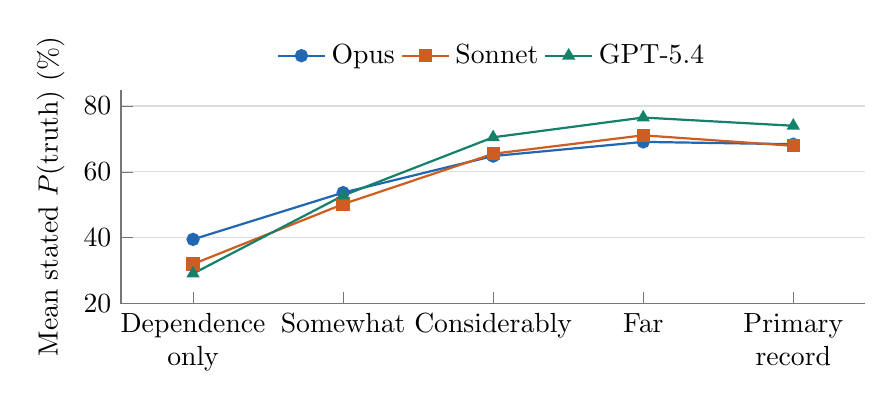
\begin{tikzpicture}
\begin{axis}[report,width=.91\textwidth,height=43mm,ymin=20,ymax=85,ytick={20,40,60,80},symbolic x coords={X3,W1,W2,W3,X5},xtick=data,xticklabels={Dependence\\only,Somewhat,Considerably,Far,Primary\\record},x tick label style={align=center,font=\normalsize},enlarge x limits=.12,ylabel={Mean stated $P(\mathrm{truth})$ (\%)},legend style={draw=none,font=\normalsize,at={(.5,1.05)},anchor=south,legend columns=3},legend cell align=left]
\addplot[opus,thick,mark=*] coordinates{(X3,39.5)(W1,53.7)(W2,64.8)(W3,69.1)(X5,68.4)};
\addplot[sonnet,thick,mark=square*] coordinates{(X3,32.0)(W1,50.2)(W2,65.5)(W3,71.1)(X5,67.9)};
\addplot[gpt,thick,mark=triangle*] coordinates{(X3,29.1)(W1,52.8)(W2,70.5)(W3,76.5)(X5,74.0)};
\legend{Opus,Sonnet,GPT-5.4}
\end{axis}
\end{tikzpicture}
\caption{Wording ladder on ten cases, with 120 trials per judge and condition. Every rung keeps the dependence note. X3 and X5 are stage-1 results for these cases. The three comparative wordings ran two days later in stage 2. Lines connect discrete conditions. Case-resampling intervals are at most $\pm$2.0 percentage points.}
\label{fig:ladder}
\end{figure}

\subsection{An abstention option rarely exposed uncertainty}
\label{sec:h6}
Few forced-choice answers were unbacked by the judge's own numbers. H6 flags an answer below the highest-probability option or a gap below ten points between the top two probabilities, after rescaling to 100. Only 30, 3 and 7 of each judge's 2,400 conflict records were flagged, all close calls. Only six had twins in the four-repeat abstention arm. None of the six abstained. This direct test is too sparse to rule H6 out generally.

All three judges can abstain. Shown one irrelevant report, they abstained in 160, 153 and 160 of 160 trials, and none abstained in A7. Yet Opus and Sonnet never abstained in their 800 conflict trials, and GPT-5.4 abstained in 9 of 800. H6 therefore found no support. The errors usually came with substantial stated support for the repeated claim, so an abstention option did not remedy them.

\section{Robustness and scope of the evidence}
\label{sec:robust}
\paragraph{Longer reports.}
With 88--96-word reports (Sonnet and GPT-5.4, ten cases), the conflict block broadly matched the short-report results. The dependence note raised $\pt$ in all ten cases for both judges. GPT-5.4 was right in 18 of 120 X3 trials, against 3 with short reports, all in T1 cases. With either quality note, both judges were right in every trial. Sonnet's A1-to-A2 rise was 13.4 points with long reports against 8.0 with short ones, larger in nine of ten cases ($p=0.011$). This comparison crosses days, so it cannot isolate a causal length effect. GPT-5.4 had little headroom: one long report already gave it 94.8\% $\pt$.

\paragraph{Targeted supplementary checks.}
With the seven echo cases left out, every direction held. On new reports for two cases, X1/X3 failures and X4/X5 successes held, while X2 improved. Sonnet made identical decisions with reasoning on and off in a two-case comparison. Only 32 of 144 enabled trials produced reasoning. All 20 X3 traces acknowledged the shared source, yet chose the repeated claim. This shows failure after acknowledgment on those trials, not a general test of reasoning models. With long reports on nine cases, Sonnet's median $\neff$ was 1.95 for rewordings and 1.97 for independent sources.

The token-probability cross-check used two models that return token probabilities, because the main judges do not. Both readings ordered the screen's three levels alike and correlated across trials (Spearman 0.83 for \href{https://openrouter.ai/meta-llama/llama-4-maverick}{Llama 4 Maverick} and 0.81 for \href{https://openrouter.ai/qwen/qwen3.6-27b}{Qwen 3.6 27B}). They part with irrelevant evidence: Qwen stated 25\% on every option while its tokens put 77\% on one number on average. This supports ordinal sensitivity on those models, not calibration or validation of the main judges' internal confidence. Details are in Appendix~\ref{app:supplement}.

\section{Discussion and limitations}
\label{sec:discussion}\label{sec:limits}
\paragraph{What the message should carry.}
Of the three fields tested in the conflict block, only a quality note made every judge right. Source-type names gave a gain that varied with the judge and quality dimension, and a dependence note moved belief and few decisions. A fourth field, an opaque source ID, ran only in the agreement block. The fields also differ in what they cost. A dependence note needs only what the system already records about which reports share a source. A quality note needs a judgment of which source is better, which is harder to produce and can be wrong.

Taken at face value, X3's note turns two-against-one into one source against one, with nothing said about which is better. The note raised the probability of the truth, but the repeated claim kept more support on average. Every quality note we showed was true, and we never tested a false one. If a false note is followed as readily, whoever writes the field could steer the orchestrator's choice. The practical recommendation therefore depends on independently established quality information.

\paragraph{Limitations.}
The judge reads fixed text in a single call. Real pipelines pass messages over several steps and tool calls, so we cannot say whether a judge-side fix changes end-to-end accuracy. Each agent reads exactly one source, reports overlap fully rather than partially, and every case is an invented single fact with four options. Every report is a rewording by one reporter. The equivalence rater, Claude Sonnet~5, is also a judge, and two judges come from one developer.

The judges ran at their providers' default temperature, and comparisons between stages carry day-to-day drift. The ladder and length arm used ten cases, the optional checks two to fifteen, and H6's direct test had six flagged twins. The main judges expose only stated numbers, whose upper scale limits the independence index. The prompt asks for the answer before the probabilities, which may tie the numbers to the answer. No control added neutral text of the same length, so generic caution from added words cannot be excluded.

\paragraph{Costs and reproducibility.}
Logged API spend came to US\$52.19 (Appendix~\ref{app:costs}). Code, cases, frozen reports, trial logs and \href{https://github.com/JasonOng0109/dsa4213-agent-project/tree/8a6de34#running-the-study}{setup instructions} are in the \href{\repo}{repository}. The \href{https://github.com/JasonOng0109/dsa4213-agent-project/blob/8a6de34/pipeline/run.py}{archived model identifiers and provider settings} specify the versions used.

The study has no human subjects and no personal data. Every entity is invented, so no output can misinform about a real institution, product or incident. Claude Code was used extensively to record decisions, draft documentation and maintain the project’s knowledge graph, and as an implementation assistant. The report was drafted with Claude’s help, then proofread and edited by all team members.

\section{Conclusion}
\label{sec:conclusion}
We asked what an orchestrator must be told before it stops counting reports and starts counting evidence. For the three judges we tested, learning that two reports share a source was not enough, and learning which source is better was. Where relative quality is independently known, the message should carry it. Future work should test false quality notes, mild notes without dependence, real tool-call messages and several aggregation steps, with more reporters and judges.
\label{main:lastpage}

\clearpage
\section*{Contribution statement}
\addcontentsline{toc}{section}{Contribution statement}
\noindent The contributions below reflect project records and subsequent report revisions. Each member should confirm and update their entry, including any additional report and presentation work, and enter an approximate share before submission. The five shares must sum to 100\%.
\begin{table}[H]
\small\renewcommand{\arraystretch}{1.25}
\begin{tabularx}{\textwidth}{@{}P{3.4cm} L P{1.4cm}@{}}
\toprule
Member & Recorded contributions & Share\\
\midrule
Ong Jia Xi\newline
(A0276092Y) & Led the project and ran paid experiments. Completed final case reviews and merges, reviewed all frozen reports, and authored M1 and M38--M40. Wrote the first draft of the final report. & \rule{.8cm}{.4pt}\%\\
Lee Kai Rong\newline
(A0287723U) & Authored nine cases (M5 and M30--M37) and reviewed 17 cases (M4, M8--M9, M16--M19, M22--M28 and M38--M40). Coordinated the corpus and ten-case subset, led the discrimination pass-mark decision, and raised post-pilot changes to the screen, ceiling rule and H6 interpretation. Supported drafting the final report. & \rule{.8cm}{.4pt}\%\\
Kathleen Pang Qi Yu\newline
(A0282219A) & Authored M4 and M22--M29 and reviewed M3, M14--M21 and M38--M40. Wrote the hedge-counting tool and drafted the revised research question. & \rule{.8cm}{.4pt}\%\\
Ee Rui Kai Rachel\newline
(A0281201X) & Authored M3 and M14--M21 and reviewed M2 and M6--M13. Led the wording-ladder sentence review. & \rule{.8cm}{.4pt}\%\\
Crystal Lai Qiaohui\newline
(A0282431L) & Authored M2 and M6--M13 and reviewed M5 and M30--M37. Led the H6 margin-cutoff decision. & \rule{.8cm}{.4pt}\%\\
\midrule
Total & & 100\%\\
\bottomrule
\end{tabularx}
\end{table}
\clearpage
\bibliographystyle{plainnat}
\bibliography{references}
\clearpage
\appendix
\setlength{\parskip}{2pt plus 1pt}
\section{Detailed protocol and experimental design}
\label{app:protocol}

\subsection{Corpus construction and report acceptance}
Five members wrote the cases under 20 authoring rules. These require comparable specificity
and scope, neutral question wording, no time markers, provenance kept apart from the content
sentence, and separate evidential routes for B, C and D. From M6 on, A's and B's type names
differ only in the case's quality dimension, and the five pilot cases keep their original
names. A static linter checked the rules a script can test, and every case from M2 on had a
reviewer other than its author.

Each round of report generation sampled six candidates at temperature 0.9, rising to 0.95 in
a second round.
A candidate had to satisfy all four acceptance requirements:
\begin{enumerate}[itemsep=2pt,topsep=3pt]
\item Claude Sonnet~5 marked all details retained, nothing added, all values unchanged,
and scope or denominator unchanged, with an equivalence score of at least 80/100.
\item Word-bigram Jaccard overlap was at most 0.70 with the source, and at most 0.50
with another retained report of that source or a source appearing in the same trial.
\item The report contained neither a word unique to its source's type name nor an
attribution phrase such as ``according to''.
\item Its length differed from the source sentence by no more than three words.
\end{enumerate}
Failed candidates were regenerated and never edited by hand, and generation stopped if a source
lacked reports after two rounds. The provenance-leak check ran again over the frozen reports
before judging.

Generation used 1,956 calls for 160 sources. Of 972 candidates, 721 passed the checks made on
each candidate alone. We kept 280 reports, two for A, three for B and one each for C and D per
case. The other 441 were surplus or too close to a report already chosen, and only two sources
needed a second round. Rejection counts, which can overlap, were 105 for length, 72 for overlap
with the source, 66 for overlap with another source's report and 12 for equivalence. In the
reading before judging, all T1 hedges survived and no case was excluded. The seven echo cases
are M3, M9, M13, M23, M28, M38 and M40. We leave them out only as a sensitivity check.

\subsection{Condition definitions and counterbalancing}
The agreement block repeats strong source B, so any change shows up in \pt{}. Source letters A--D name authored sources, while the displayed agent letters name
rotating report slots. Table~\ref{tab:conditions} lists every condition, and
Table~\ref{tab:arms} lists what ran.

\begin{table}[H]
\centering\small
\caption{The 13 conditions and the wording ladder. Agent labels (Agent A, B, C) name report
slots and rotate with the order, and they are unrelated to the source names A--D. A message is one
``Agent \dots{} says'' line of the single prompt. Appendix~\ref{app:prompts} shows example
prompts in full.}
\label{tab:conditions}
\begin{tabularx}{\textwidth}{@{}l c c c l L@{}}
\toprule
& Reports & Messages & Agents & Sources & What the judge is told besides the reports\\
\midrule
A0 & 0 & 0 & 0 & none & nothing. The question alone gives the judge's prior\\
A1 & 1 & 1 & 1 & B & nothing\\
A2 & 3 & 1 & 1 & B & nothing. Three rewordings of B are joined into one message\\
A3 & 3 & 3 & 1 & B & nothing. Lines labelled ``Agent A, report 1'' to ``report 3''\\
A4 & 3 & 3 & 3 & B & nothing\\
A5 & 3 & 3 & 3 & B & an opaque source ID, ``(source: S-001)'', on every report\\
A6 & 3 & 3 & 3 & B & A5, plus a dependence note: all ``obtained their information from the same underlying source (S-001)''\\
A7 & 3 & 3 & 3 & B, C, D & nothing\\
\midrule
X1 & 3 & 3 & 3 & A, A, B & nothing\\
X2 & 3 & 3 & 3 & A, A, B & each report's source type name\\
X3 & 3 & 3 & 3 & A, A, B & a dependence note: the two A reports ``obtained their information from the same underlying source'', while B's ``comes from a different, independent source''\\
X4 & 3 & 3 & 3 & A, A, B & a quality note: B's source ``is a primary, authoritative record; the other reports rest on secondhand or unofficial material''\\
X5 & 3 & 3 & 3 & A, A, B & X3's note, plus a quality note: B's source ``is a primary, authoritative record; the source shared by'' the other two ``is a secondhand or unofficial one''\\
W1--W3 & 3 & 3 & 3 & A, A, B & X3's note, plus a softened quality note: B's source ``is somewhat / considerably / far more reliable than the source shared by'' the other two\\
\bottomrule
\end{tabularx}
\end{table}
The conflict block's 12 repeats pair every answer position with every independent-report
slot once, and every answer position with every wrong-claim offset once. Agreement uses
six repeats under the same fixed schedule in every condition. The abstention arm's four repeats
put the truth in each answer position once. These repeats measure response stability and reduce
position imbalance.

The length arm embeds each report in one of three authored sets of neutral filler. Filler
is assigned by slot and mentions no answer option. Each long report has 88--96 words, the
longest within a trial is at most 1.10 times the shortest, and the report sentence rotates
among the start, middle and end. The arm uses Sonnet and GPT-5.4, one judge per developer. The ten-case subset is M1--M6, M14, M22, M30 and M38. Under
a selection rule that predates the pilot, every domain appears at least three times, every
quality dimension at least twice, and three cases are T2.

The abstention arm adds ``Cannot be determined from the evidence provided'' to X1--X5,
A7 and P0. P0 is an irrelevant report that checks whether the judge can abstain. A7
checks whether it abstains despite three agreeing independent sources. Before the main run we
fixed two labels. A judge that abstains in fewer than half of its P0 trials ``abstains nowhere'',
and one that abstains in at least half of its A7 trials ``abstains everywhere''.

\begin{table}[H]
\centering\small
\caption{What ran. The short arm and the length arm each have an agreement entry and a
conflict entry. We fixed the design of each optional sub-experiment before it ran.}
\label{tab:arms}
\begin{tabular}{@{}l l c l c r@{}}
\toprule
Entry & Conditions & Repeats & Judges & Cases & Trials\\
\midrule
\multicolumn{6}{@{}l}{\emph{Main run, stage 1}}\\
Agreement & A0--A7 & 6 & all three & 40 & 5,760\\
Conflict & X1--X5 & 12 & all three & 40 & 7,200\\
Abstention & X1--X5, A7, P0 & 4 & all three & 40 & 3,360\\
Confidence screen & P0, P1, P2 & 4 & all three & 40 & 1,440\\
\multicolumn{6}{@{}l}{\emph{Main run, stage 2}}\\
Wording ladder & W1--W3 & 12 & all three & 10 & 1,080\\
Length, agreement & A1, A2, long & 6 & Sonnet, GPT-5.4 & 10 & 240\\
Length, conflict & X1--X5, long & 12 & Sonnet, GPT-5.4 & 10 & 1,200\\
\multicolumn{5}{@{}l}{Main run in total} & 20,280\\
\midrule
\multicolumn{6}{@{}l}{\emph{Optional sub-experiments}}\\
Reasoning off and on & X1, X3, X5 (short, long) & 12 & Sonnet & 2 & 288\\
Second report set & X1--X5 & 12 & all three & 2 & 360\\
Stated vs.\ token probabilities & P0, P1, P2 & 4 & Qwen, Llama & 16$^{a}$ & 384\\
Independence index, long & A4, A6, A7, long & 6 & Sonnet & 9 & 162\\
\bottomrule
\end{tabular}\\[1mm]
\parbox{0.92\textwidth}{\footnotesize $^{a}$We read 15 cases. M10's 24 trials were set aside
because its option values are also option numbers, and M12 was judged in its place.}
\end{table}
\subsection{Judging, validation, and analysis details}
\label{app:analysis}
The judges were pinned to Claude Platform on AWS for Claude and to OpenAI for GPT-5.4. Records
keep the raw reply, parse, provider, token usage and cost. The equivalence rater, like the
judges, ran at its provider's default temperature. A six-call probe of identical prompts
returned the same answer six times for Sonnet and five times for Opus and GPT-5.4, so responses
were consistent, though not provably deterministic.

Stage~1's 18 imperfect records were 15 probability sums outside 90--110, two answers naming
no option and one missing option probability. With the one parse failure, all were in A0, P0
or P1. No completed main-run call changed provider or used reasoning.

Decision stability is the share of a cell's repeats (one judge, case and condition) that give
its most common answer. Under random answering it would be 0.41 for 12 repeats, 0.47 for six
and 0.53 for four. Conflict stability averaged 0.96--0.97, all 12 answers agreed in 168--178
of the 200 cells per judge, and the A1--A7 values were 1.00.

For the confidence screen, each case contributes its mean over four rotations to Page's test,
with a planned one-sided threshold of 0.05. P0 supplies irrelevant text, P1 rules out two
options and keeps the truth, and P2 uses B's first frozen report. Within-condition
discrimination was below 0.5 in X1 and X3 (AUROC 0.01--0.37), because the judges were surer of
their wrong answers, which follow the two agreeing reports, than of their right ones. X2
AUROCs were 0.71, 0.37 and 0.57 for Opus, Sonnet and GPT-5.4.

Equation~\eqref{eq:neff} adapts correlation-neglect reasoning
\citep{demarzo2003persuasion,enke2019correlation}. Its reference values of one for repeated
reports and three for independent sources assume additive log-likelihood contributions of
equal strength, a common prior and a faithful probability scale, so they are benchmarks under
that model. We clip means outside 1--99\% and report them as bounds. Ceiling flags affect 0, 1
and 35 cases for Opus, Sonnet and GPT-5.4. Even without clipping, a compressed scale can hide
differences. With Opus's mean A0 and A1 (25.8 and 77.4), three sources adding in log-odds would
put \pt{} at 99.7, but Opus never stated more than 97 in any of its 720 A3, A4 and A7 trials,
and its most common value was 94 in both A4 and A7. At 97 its index reaches only about 2, so
the reference value of 3 for A7 was out of reach, and the small A7 $-$ A4 gap is partly a
ceiling effect. Sonnet stated 100 in about a quarter of its A4 and A7 trials (54 and 62 of 240).

Sign tests over cases count positive and negative paired changes and omit ties. The 95\%
bootstrap intervals resample whole cases 10,000 times with seed 4213. Reported means follow the
scorer, which rounds within-case means to one decimal before averaging cases, so direct averages
of raw trials can differ by 0.1 percentage points. Counts and conclusions are unaffected. We apply
no correction for multiple comparisons.

A flagged H6 trial's abstention twin is the abstention-arm trial with the same case, condition
and repeat. The planned contrast compares abstention in the twins of flagged trials with
abstention in the twins of the others, within condition, combined with a Mantel--Haenszel
difference and read alongside P0 and A7. Only six flagged trials have twins, four for Opus and
two for GPT-5.4, so this contrast has little power to show the absence of an effect.

\section{Hypotheses and interpretation}
\label{app:hypotheses}
Table~\ref{tab:hypotheses} gives the hypotheses in their wording from before data collection,
and Table~\ref{tab:verdicts} sets each result beside the patterns fixed at that time. Those
patterns set no number for an unchanged decision rate, so Section~\ref{sec:conflict} reads H3
with sign tests over cases. H1 and H2 extend prior findings to paraphrased reports.

\begin{table}[H]
\centering\small
\caption{The six hypotheses and the contrast that tests each. Section~\ref{sec:conditions}
defines the conditions.}
\label{tab:hypotheses}
\begin{tabularx}{\textwidth}{@{}l L P{3.2cm} P{2.6cm}@{}}
\toprule
& Hypothesis & Tested by & Status\\
\midrule
H1 & Correlated repetition raises the orchestrator's confidence and can beat a single
better-sourced report & A1 $\to$ A4 and the X1 level & expected from prior work\\
H2 & The rise is driven by report redundancy and segmentation, not by distinct agent
identities & A1 to A4 step by step and A4 against A7 & expected from prior work\\
H3 & Stating that two reports share a source shifts belief but does not change the decision
& X1 $\to$ X3 & primary\\
H4 & Stating relative source quality does change the decision & X3 against X4 and X5, plus the
wording ladder & primary\\
H5 & Judges infer quality from named source types without being told & X1 $\to$ X2 &
secondary\\
H6 & Forced choice conceals belief. Where a judge's stated probabilities do not identify its
answer, an explicit ``cannot be determined'' option will be taken when offered & the
abstention arm & primary\\
\bottomrule
\end{tabularx}
\end{table}
\begin{table}[H]
\centering\footnotesize
\caption{Each hypothesis read against the patterns fixed before any data. A small or
non-significant decision change does not establish equivalence.}
\label{tab:verdicts}
\begin{tabularx}{\textwidth}{@{}P{0.55cm} P{3.3cm} P{3.1cm} L@{}}
\toprule
& Predicted evidence & Alternative pattern & Result\\
\midrule
H1 & Repetition raises confidence. A repeated weak claim defeats a single strong claim. &
An effect confined to one domain or report position. &
\textbf{Support} in this corpus. A1 to A4 raises \pt{} in all 40 cases for every judge, and X1
is right in 1, 2 and 26 of 480.\\
\addlinespace
H2 & A3 and A4 exceed A2 and differ little. & A larger A1 to A2 increase at long length. &
\textbf{Support} with short reports, where segmentation outweighs agent identity.
\textbf{Alternative pattern} for Sonnet with long reports (+13.4 against +8.0 points), though
the comparison crosses days. GPT-5.4 has little headroom, and Opus was not tested.\\
\addlinespace
H3 & Dependence disclosure raises \pt{} without changing decisions. & Decision changes
occur only where a mild textual cue survives. &
Belief rose for every judge. \textbf{Support} for Sonnet, and for GPT-5.4 with short reports.
\textbf{Alternative pattern} for Opus (1 to 63 right, all in T1) and for GPT-5.4 with long
reports (18 of 120 right, all in T1).\\
\addlinespace
H4 & Quality disclosure changes decisions beyond dependence disclosure. & Decisions change
only under the strongest wording. &
\textbf{Support} for true notes. X4 and X5 are right in 480 of 480 for every judge, and
``somewhat'' in 120, 91 and 120 of 120. All 29 of Sonnet's wrong W1 answers named A's claim, 16
of them in the three T2 cases. The ladder rules out an effect of the strongest wording alone but
cannot separate compliance from weighing the evidence.\\
\addlinespace
H5 & Named source types improve accuracy. & Gains require a familiar real institution. &
\textbf{Support}, varying by judge and dimension. Gains remain outside the eight
familiarity-coded cases, though familiarity and authority are confounded.\\
\addlinespace
H6 & Abstention concentrates where the judge's numbers do not support its answer. &
A judge abstains indiscriminately or cannot abstain. &
\textbf{No support}. None of the six flagged twins abstains, and GPT-5.4's contrast gives
$+0.00$ on two twins. P0 and A7 show selective use of abstention, but six twins are too few to
rule out the predicted relationship.\\
\bottomrule
\end{tabularx}
\end{table}

\section{Supplementary results and sensitivity checks}
\label{app:supplement}
\subsection{Source-type effects and report length}
Table~\ref{tab:dimension} breaks X2 down by quality dimension. This breakdown is descriptive and
sits outside the hypotheses. All judges did best on method cases and worst on primary-source
cases. In eight cases, B's type names a public or official body that A's does not. In the other
32 cases, right decisions rose in 30, 19 and 25 cases and fell in none (one-sided sign tests,
$p<0.0001$). Seven of the eight familiar cases are authority cases, so familiarity and that
dimension cannot be told apart. X2 also shows the same type name on both of A's reports, a hint
that they share a source. Since X3's explicit dependence note moved few decisions, that hint is
unlikely to explain the gain.

\begin{table}[H]
\centering\small
\caption{Right decisions in X2 by the case's quality dimension, of 120 trials (ten cases, 12
repeats).}
\label{tab:dimension}
\begin{tabular}{@{}lrrrr@{}}
\toprule
& Authority & Directness & Method & Primary source\\
\midrule
Claude Opus 5 & 106 & 93 & 117 & 87\\
Claude Sonnet 5 & 56 & 59 & 66 & 12\\
GPT-5.4 & 84 & 76 & 99 & 24\\
\bottomrule
\end{tabular}
\end{table}
\begin{table}[H]
\centering\small
\caption{Length-arm details on the ten-case subset. S and L denote short and long reports,
judged on different days. Right decisions are of 120 per cell.}
\label{tab:length}
\begin{tabular}{@{}lrrrr@{}}
\toprule
& Sonnet S & Sonnet L & GPT-5.4 S & GPT-5.4 L\\
\midrule
Right, X1 & 0 & 1 & 2 & 4\\
Right, X2 & 52 & 36 & 87 & 74\\
Right, X3 & 1 & 1 & 3 & 18\\
Right, X4 & 120 & 120 & 120 & 120\\
Right, X5 & 120 & 120 & 120 & 120\\
\midrule
Mean \pt{}, X1 & 20.3 & 19.8 & 21.4 & 21.9\\
Mean \pt{}, X3 & 32.0 & 27.5 & 29.1 & 30.3\\
Mean \pt{}, A1 & 75.8 & 78.3 & 90.3 & 94.8\\
Mean \pt{}, A2 & 83.8 & 91.7 & 96.2 & 95.6\\
A1 to A2 increase (points) & 8.0 & 13.4 & 5.9 & 0.8\\
\bottomrule
\end{tabular}
\end{table}

Table~\ref{tab:length} gives the length arm's details. GPT-5.4's long X3 beat its short X3 in
seven cases and fell behind in none ($p=0.008$). Sonnet's larger A1 to A2 rise holds in seven
of eight cases without the subset's echo cases ($p=0.035$). The rise fits a contribution from
report length, but short and long prompts were judged on different days. On 24 identical A0
prompts shared by the pilot and main run, 22 decisions matched for each judge, and mean absolute
\pt{} shifts were 0.5--2.7 points, with Sonnet at 2.7. These A0 comparisons do not directly
estimate drift in the length contrast.

\subsection{Optional experiments and echo-case sensitivity}
Table~\ref{tab:robust} lists these checks.

\begin{table}[H]
\centering\small
\caption{Sensitivity and optional checks. Each finding is limited to the stated cases and
models.}
\label{tab:robust}
\begin{tabularx}{\textwidth}{@{}P{3.2cm} L@{}}
\toprule
Check & Evidence and qualification\\
\midrule
Exclude seven echo cases &
Every direction holds across 33 cases. X2 is right in 350, 156 and 243 of 396 for Opus,
Sonnet and GPT-5.4. Without M3 and M38, Sonnet's A1 to A2 rise is 8.7 points short and 13.7
long.\\
\addlinespace
Second report set, M1 and M2 &
Every judge stays at 0 of 24 in X1 and X3 and 24 of 24 in X4 and X5. X2 stays at 24 for Opus
and moves from 9 to 13 for Sonnet and from 22 to 24 for GPT-5.4. \pt{} moves by at most 7.5
points in any case and condition. The runs fell on different days.\\
\addlinespace
Reasoning allowed, Sonnet, M1 and M2 &
Decisions match reasoning-off trials at both lengths, with X1 and X3 right in 0 of 48 each
and X5 in 48 of 48. Only 32 of 144 trials produce reasoning text, so the traces describe those
trials alone.\\
\addlinespace
Stated and token confidence, 15 cases &
Llama~4 Maverick and Qwen~3.6 27B both order P0 $<$ P1 $<$ P2 in both measures
(Page's $p<0.0001$). Llama's trial-level Spearman correlation is 0.83 and Qwen's is 0.81.
Within P1 they are 0.79 and 0.76. Qwen states 25\% per option at P0, while its largest
token probability averages 76.9\%.\\
\addlinespace
Long-report index, Sonnet, nine cases &
Median $\neff$ is 1.95 for A4 and 1.97 for A7 (short: 1.86 and 1.79 on the same cases).
The median paired A4 minus A6 difference is 0.47 (short: 0.23). M38 is omitted because
its long A7 construction falls one word below the band. Conditions span different days.\\
\bottomrule
\end{tabularx}
\end{table}

The confidence cross-check ran 16 cases and uses 15. In M10 the answer values 2--5 are also
option numbers, so a returned digit is ambiguous, and M12 took its place. The 15 cases give 360
trials, with token probabilities read at the answer digit.

Two fresh Claude agents coded the 32 nonempty reasoning traces independently, shuffled and blind
to case, condition and result. They agreed on 31, and a team member settled the last, an X5
trace, as noticing the dependence. The X3 result does not depend on that call. The other 112
trials hold no reasoning text. Section~\ref{sec:discussion} quotes trials
\texttt{M2\_X3\_reasoning-on-short\_run1} and \texttt{M2\_X5\_reasoning-on-short\_run5}.

\clearpage
\section{Deviations and costs}
\label{app:departures}
The pilot used M1--M5 and 3,420 judge trials. It was a design check and is not pooled with
the main study. Table~\ref{tab:departures} lists what changed and what followed.

\begin{small}
\begin{xltabular}{\textwidth}{@{}P{3.2cm} L L@{}}
\caption{Departures from the planned protocol and their effects.}\label{tab:departures}\\
\toprule
Original plan & What changed & Consequence\\
\midrule
\endhead
Ordering and AUROC above 0.5 gate stated probabilities &
After the pilot and before the main run, only ordering decides. In conflict cells,
discrimination measures how sure a judge is of the repeated wrong claim, which is the effect
under study. &
Sonnet and GPT-5.4 would have failed the original rule. Decisions are unaffected.\\
\addlinespace
Temperature 0 for all judges &
Temperature 0 is sent, but no judge endpoint accepts it. We found this after stage~1. &
Provider defaults apply. Repeated calls and cross-day comparisons cannot be treated as
deterministic or free of drift.\\
\addlinespace
Three authored screen sentences &
P0 uses filler, P1 an authored exclusion statement, and P2 B's first frozen report. &
P2 still names the answer, but it is reporter output.\\
\addlinespace
H6 interpreted against A7 alone &
P0 and the selective-abstention cut-offs were added after the pilot and before the main run. &
The controls establish that judges can abstain selectively, but six flagged twins still limit
the direct H6 test.\\
\addlinespace
Point estimates for the independence index &
The scorer's original 1--99\% clipping remains, but clipped means are reported as bounds
following the pilot. &
GPT-5.4's index is a bound in 35 of 40 cases.\\
\addlinespace
Calibration summaries where spread permits &
Brier scores were not computed. Analysis uses within-judge differences and ranks. &
No hypothesis reading uses them.\\
\addlinespace
Initial research-question wording &
After the TA's feedback, the wording names the aggregation step and the lost source record. &
The experimental design is unchanged.\\
\bottomrule
\end{xltabular}
\end{small}

The stopped long-conflict log is kept and left out of scoring. In the second report set, two
regenerated reports of D repeated existing wording, which cannot affect the check because it uses
only A and B.

\subsection{API costs}
\label{app:costs}
Table~\ref{tab:costs} lists the logged spend. The total covers the pilot, the stopped first attempt
and the optional experiments as well as the main study.

\begin{table}[H]
\centering\small
\caption{Logged API spend in US dollars. Judge costs are the sum of each log's per-call costs,
and generation costs are the fall in the account balance while generation ran.}
\label{tab:costs}
\begin{tabular}{@{}l r r@{}}
\toprule
Item & Calls & Spent\\
\midrule
Pilot, M1--M5: judging & 3,420 & 6.72\\
P0 check after the pilot & 60 & 0.12\\
Stage 1: generation and judging & 19,716 & 36.78\\
Stage 2: judging & 2,520 & 5.25\\
Stage 2: stopped first try of one entry & 762 & 1.60\\
Optional sub-experiments, with 96 report calls & 1,290 & 1.72\\
\midrule
Total logged & 27,768 & 52.19\\
\bottomrule
\end{tabular}
\end{table}

\clearpage
\section{Prompt templates and logged replies}
\label{app:prompts}

The A6 example gives the complete prompt. The following examples specify the changed
content under the same template, with complete logged replies. The two block examples use
case M1, repeat~1. The H6 mismatch example uses M20. Replies are copied from the trial logs. The system message for every
judge call is ``You are a careful, literal reader of the reports you are given.''

\subsection{Agreement block: A6}
\label{app:a6}
This is trial \texttt{M1\_A6\_short\_run1}. The truth is 15\%.
\begin{Verbatim}[fontsize=\footnotesize, breaklines=true, frame=single, framesep=2mm]
You are asked to answer a factual question based on reports from others.
Read all reports below, then give your answer.

Question: What percentage of the final ME2103 grade comes from the lab logbook?
Possible answers:
  1. 15%
  2. 25%
  3. 10%
  4. 30%

Agent A (source: S-001) says: For module ME2103, the lab logbook contributes 15% toward the final grade.
Agent B (source: S-001) says: The final grade for module ME2103 includes a 15% contribution from the lab logbook.
Agent C (source: S-001) says: The lab logbook is worth 15% of the overall grade for module ME2103.
Note: Agent A, Agent B, and Agent C all obtained their information from the same underlying source (S-001).

Respond with ONLY a JSON object in exactly this format, nothing else:
{"answer": "<one of the possible answers, verbatim>",
 "p": {"<answer text>": <integer 0-100>, ...}}

"p" must give a probability for every possible answer listed above, using the
answer text as the key, and the values must sum to 100.

Do not include any explanation or reasoning -- output only the JSON object.
\end{Verbatim}
\begin{Verbatim}[fontsize=\footnotesize, breaklines=true]
Claude Opus 5:   {"answer": "15%", "p": {"15%": 88, "25%": 4, "10%": 5, "30%": 3}}
Claude Sonnet 5: {"answer": "15%", "p": {"15%": 90, "25%": 4, "10%": 3, "30%": 3}}
GPT-5.4:         {"answer":"15%","p":{"15%":100,"25%":0,"10%":0,"30%":0}}
\end{Verbatim}

\clearpage
\subsection{Conflict block: X3, and what the other conditions change}
\label{app:x3}
This is trial \texttt{M1\_X3\_short\_run1}. The truth is 15\%, A's claim is 25\%, and M1
is a T2 case. In this trial the Agent A slot holds the report of strong source B. The prompt is
the same as above down to the options, and the reports and note are as follows.
\begin{Verbatim}[fontsize=\footnotesize, breaklines=true, frame=single, framesep=2mm]
Agent A says: The final grade for module ME2103 includes a 15% contribution from the lab logbook.
Agent B says: Twenty-five percent of the final module grade for ME2103 is derived from the lab logbook.
Agent C says: The lab logbook accounts for 25% of the final module grade for ME2103.
Note: Agent B and Agent C obtained their information from the same underlying source; Agent A's information comes from a different, independent source.
\end{Verbatim}
\begin{Verbatim}[fontsize=\footnotesize, breaklines=true]
Claude Opus 5:   {"answer": "25%", "p": {"15%": 38, "25%": 57, "10%": 3, "30%": 2}}
Claude Sonnet 5: {"answer": "25%", "p": {"15%": 30, "25%": 60, "10%": 5, "30%": 5}}
GPT-5.4:         {"answer":"25%","p":{"15%":29,"25%":67,"10%":2,"30%":2}}
\end{Verbatim}
All three judges chose the repeated claim and put 29 to 38 on the truth. In the same
repeat, the other conditions keep these reports and change only the following.
X1 has no note. X2 has no note and labels each report with its source type.
\begin{Verbatim}[fontsize=\footnotesize, breaklines=true]
Agent A (source: ME2103 assessment brief, section 4) says: ...
Agent B (source: student-run module wiki page) says: ...
Agent C (source: student-run module wiki page) says: ...
\end{Verbatim}
X4's note is ``Note: Agent A's source is a primary, authoritative record; the other reports rest
on secondhand or unofficial material.'' X5's note is X3's followed by ``Agent A's source is a
primary, authoritative record; the source shared by Agent B and Agent C is a secondhand or
unofficial one.'' W1's note is X3's followed by ``Agent A's source is somewhat more reliable
than the source shared by Agent B and Agent C.'' W2 and W3 replace ``somewhat'' with
``considerably'' and ``far''. In the abstention arm, the following line precedes the final
instruction.
\begin{Verbatim}[fontsize=\footnotesize, breaklines=true]
If the reports do not determine the answer, you may instead answer exactly "Cannot be
determined from the evidence provided", still giving "p" over the numbered answers above.
\end{Verbatim}

\clearpage
\subsection{An answer whose own numbers favour another option}
\label{app:h6}
Trial \texttt{M20\_P1\_screen\_run4} is the confidence screen's middle level, in the rotation
that lists the truth last. The truth is 48 minutes. The prompt is the template above with
the following content.
\begin{Verbatim}[fontsize=\footnotesize, breaklines=true, frame=single, framesep=2mm]
Question: What is the continuous runtime of the AeroGlide T5 vacuum cleaner on its standard power setting?
Possible answers:
  1. 41 minutes
  2. 34 minutes
  3. 55 minutes
  4. 48 minutes

Agent A says: The continuous runtime of the AeroGlide T5 vacuum cleaner on its standard power setting is between 37 minutes and 52 minutes.
\end{Verbatim}
\begin{Verbatim}[fontsize=\footnotesize, breaklines=true]
Claude Opus 5:   {"answer": "41 minutes", "p": {"41 minutes": 40, "34 minutes": 5, "55 minutes": 5, "48 minutes": 50}}
Claude Sonnet 5: {"answer": "48 minutes", "p": {"41 minutes": 20, "34 minutes": 5, "55 minutes": 5, "48 minutes": 70}}
GPT-5.4:         {"answer":"48 minutes","p":{"41 minutes":21,"34 minutes":8,"55 minutes":4,"48 minutes":67}}
\end{Verbatim}
The report leaves two options, 41 and 48 minutes, each four minutes inside a bound. Opus answered
41 minutes, the first of the two in the list, and then put 50 on the truth and 40 on 41 minutes.
Its stated belief favours one answer and its decision names another, the strongest mismatch H6
describes. No such record occurred in the forced-choice conflict block.

\end{document}
